\documentclass{report}
\usepackage[pdftex]{graphicx}
\usepackage{sidecap}
\usepackage{fancyhdr}
\usepackage{lscape}
\usepackage[francais]{babel} 
\usepackage[absolute]{textpos}
\usepackage{amssymb}


\usepackage[utf8]{inputenc}  
\usepackage[T1]{fontenc}


\title{Rapport de labo d'\'electronique: \\ Mesures ARDUINO}
\author{Groupe ?: \\ Mattens Simon; Dom Eduardo \\ BA2 Info}
\date{Labo r\'ealis\'e le 14 mai 2018}

\pagestyle{fancy}
\lhead{Groupe ?: Mattens S. ; Dom E.}
\rhead{BA2 Info}
\cfoot{\thepage}
\begin{document}
\maketitle

\section*{1 Introduction}
Le but de ce cette scéance est de nous familiariser à l'utilisation de systèmes basés sur l'interface ARDUINO et sa gestion par PC. Nous allons réaliser des fonctions logiques en électronique programmable et nous testerons différents circuits proposés dans le starter kit.\\

\section*{2 R\'esum\'e Th\'eorique}
ARDUINO est souvent défini comme une plate-forme de prototypage open-source d'objets interactifs constituée d'une carte électronique et d'un environnement de programation IDE. Cet environnement matériel et logiciel permet de formuler et d'expérimenter des projets grâce aux nombreuses ressoucres disonibles en ligne.\\
C'est un exemple d'interface entre le monde réel analogique et le monde numérique.\\
\\La carte ARDUINO UNO est un circuit intégré associé à des entrées et sorties qui permettent à l'utilisateur de brancher différents types d'éléments externes : \\
\\
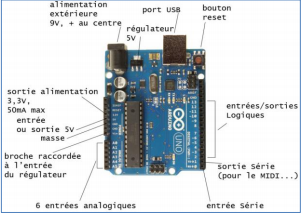
\includegraphics{Arduino.png}
 
\section*{3 Dispositif exp\'erimental}
\begin{itemize}
\item Plaquette de connexions Breadboard et divers fils de branchement.
\item Divers composants électroniques : resistances, LEDs, écran-afficheur LCD, servomoteur,...
\item Carte ARDUINO UNO.
\item Câble USB-ARDUINO.
\item Pc avec logiciel ARDUINO installé avec divers exemples à tester.\\
\end{itemize}
\newpage
Nous avons testé le projet "Spaceship interface" ainsi que le projet "Love-o-meter".\\
\\
\textbf{Schéma du projet Spaceship interface: }
\begin{figure}[h!]
\centering
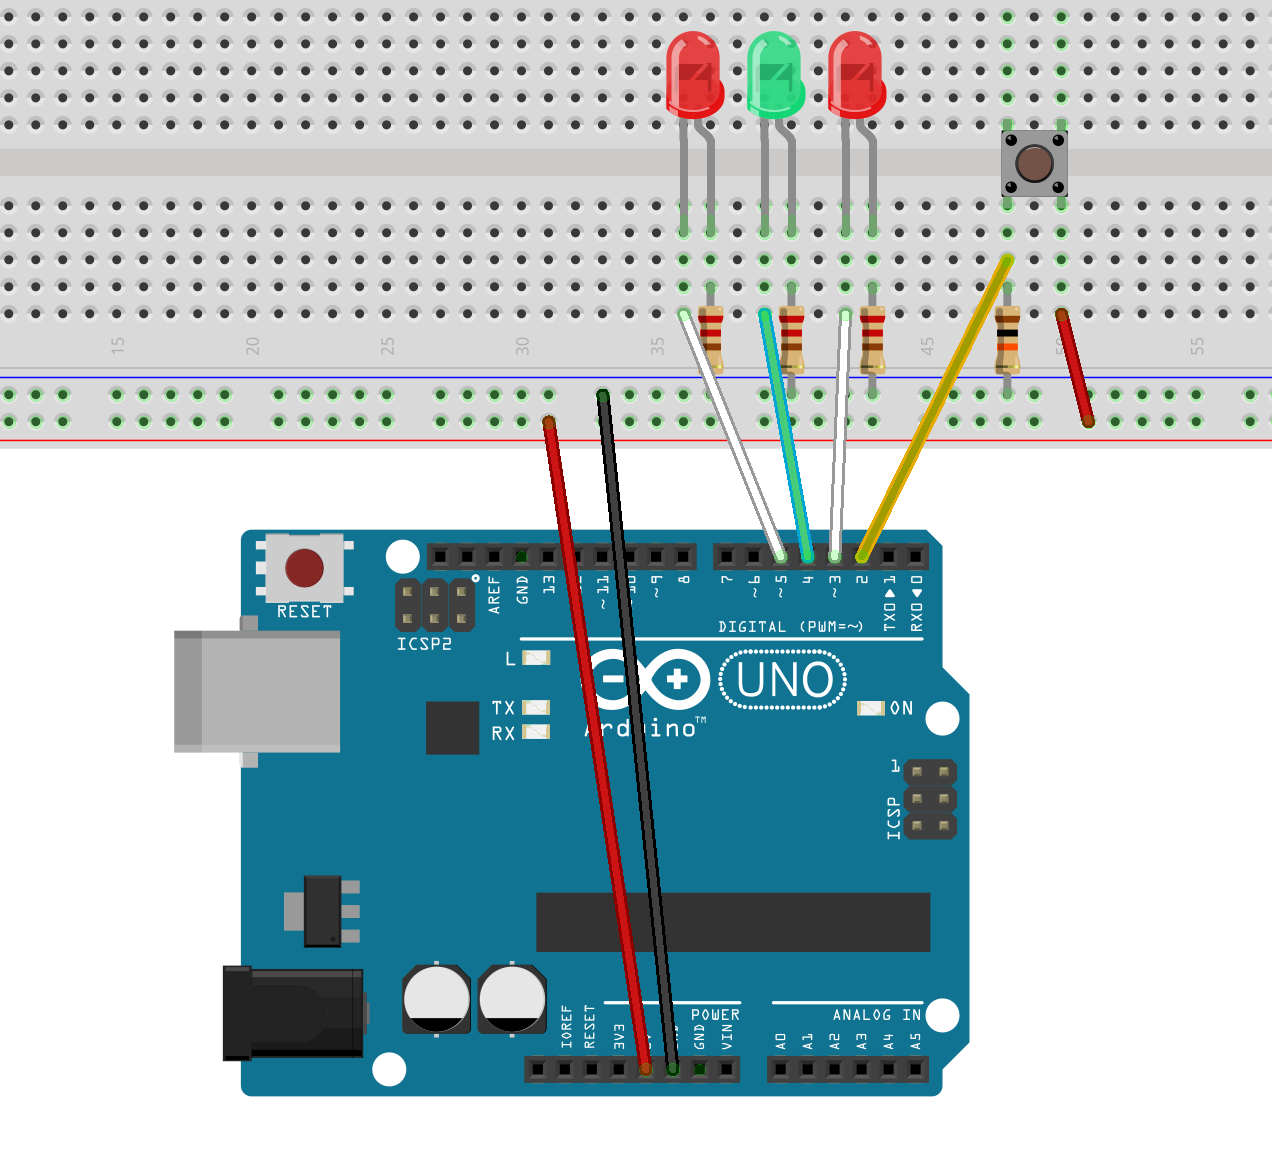
\includegraphics[scale=0.25]{SpaceInt.png}
\end{figure}
\newpage
\textbf{Schéma du projet Love-o-meter: }
\begin{figure}[h!]
\centering
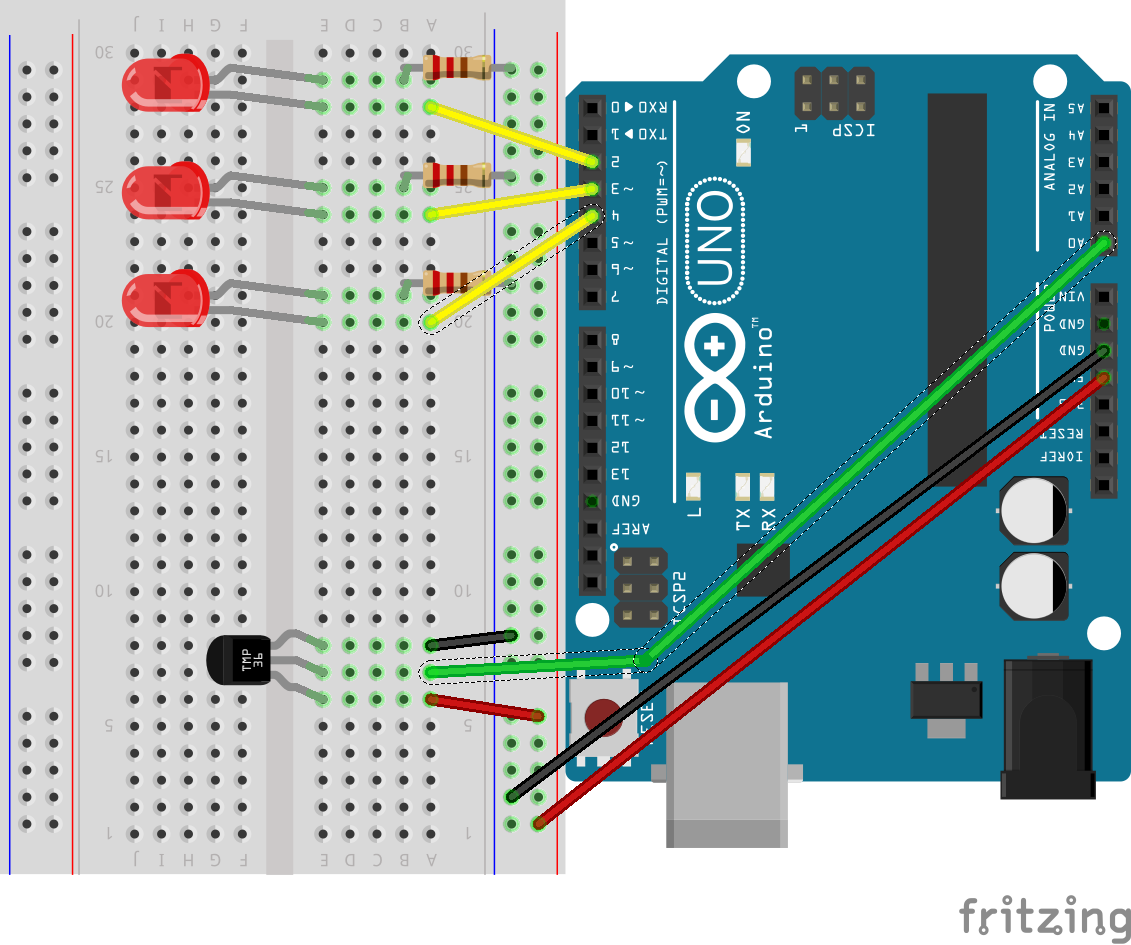
\includegraphics[scale=0.25]{Love.png}
\end{figure}
\newpage
Il nous ait demandé de faire le circuit suivant afin de simuler des fonctions logiques:\\
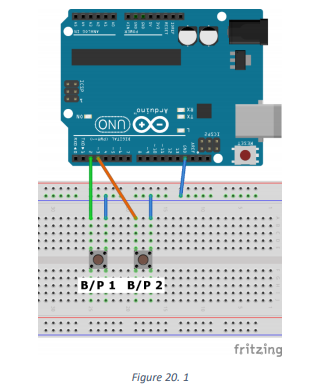
\includegraphics{FctLog.png} 



\section*{4 Prise des mesures et résultats}

\subsection*{4.1 Spaceship interface}
Les 2 LEDs rouges clignotent et lorsqu'on appuie sur l'interrupteur elles s'éteignent et la LED verte reste allumée.

\subsection*{4.2 Love-o-meter}
Au plus la température du termomètre augmente au plus le nombre de LEDs allumées augmente.(Elles sont toutes éteintes lors du début de l'expérience).

\subsection*{4.3 Simulation de fonctions logiques}

\subsubsection*{4.3.1 Fonction monostable}
Lorsqu'on appuie sur l'interrupteur BP1, une LED orange s'allume brievement sur l'ARDUINO UNO (+/- 2 secondes) et s'éteins après. \\ Lorsqu'on appuie sur l'interrupetur BP2 rien ne se passe.

\subsubsection*{4.3.1 Fonction bistable}
Lorsqu'on appuie sur l'interrupteur BP1, une LED orange s'allume sur l'ARDUINO UNO et ne s'éteint pas. \\ Lorsqu'on appuie sur l'interrupetur BP2, la LED orange qui est allumée sur l'ARDUINO UNO s'éteint.

\subsubsection*{4.3.1 Fonction OR}
Lorsqu'on appuie sur l'interrupteur BP1, une LED orange s'allume brièvement sur l'ARDUINO UNO. \\ Lorsqu'on appuie sur l'interrupteur BP2, une LED orange s'allume brièvement sur l'ARDUINO UNO.\\ Et lorsqu'on appuie sur les deux interrupteurs en même temps, une LED orange s'allume brièvement sur l'ARDUINO UNO.

\subsubsection*{4.3.1 Fonction AND}
Pour que la LED orange de l'ARDUINO UNO s'allume il faut que les 2 interrupteurs BP1 et BP2 soient appuyés en même temps.

\subsubsection*{4.3.1 Fonction XOR}
La LED orange de l'ARDUINO UNO s'allume si soit nous appuyons seulement sur l'interrupteur BP1 ou soit sur l'interrupteur BP2. La LED reste éteinte si on appuie sur les deux interrupteurs en même temps.

\section*{5 Analyse des r\'esultats}
En ce qui concerne le projet "LoveoMeter", le fait que plusieurs LEDs s'allument grâce à l'augmentation de chaleur est du à la conductivité du cristal qui augmente avec la chaleur.\\
Nous remarquons que  tous nos résultats de la simulation de fonctions logiques concordent avec les résultats attendus.

\section*{6 Conclusion}

Durant cette s\'eance de laboratoire, nous avons pu nous familiariser avec ARDUINO et tester différents projets disponibles.\\
Nous avons pu remarquer qu'il est possible d'implémenter et tester des fonctions logiques avec ARDUINO.


\end{document}